\chapter{Construction}
\minitoc

\section{Importation d'un dump}
\subsection{Définition}
Il s'agit d'une sauvegarde pouvant concerner la structure de la base de données, ses données, ou les deux.

\subsection{Importation}
\begin{enumerate}
    \item Depuis l'éditeur \textit{query tool}, ouvrir le \textit{dump} en \texttt{.sql} et exécuter le fichier.
    \item On définit le chemin de recherche dans la BDD comme le chemin public :
    \begin{lstlisting}[language=SQL]
    SET search_path = 'public'
    \end{lstlisting}
\end{enumerate}

\subsection{Modèle relationnel}
Le modèle relationnel de la BDD importée est le suivant :
\begin{figure}[H]
    \centering
    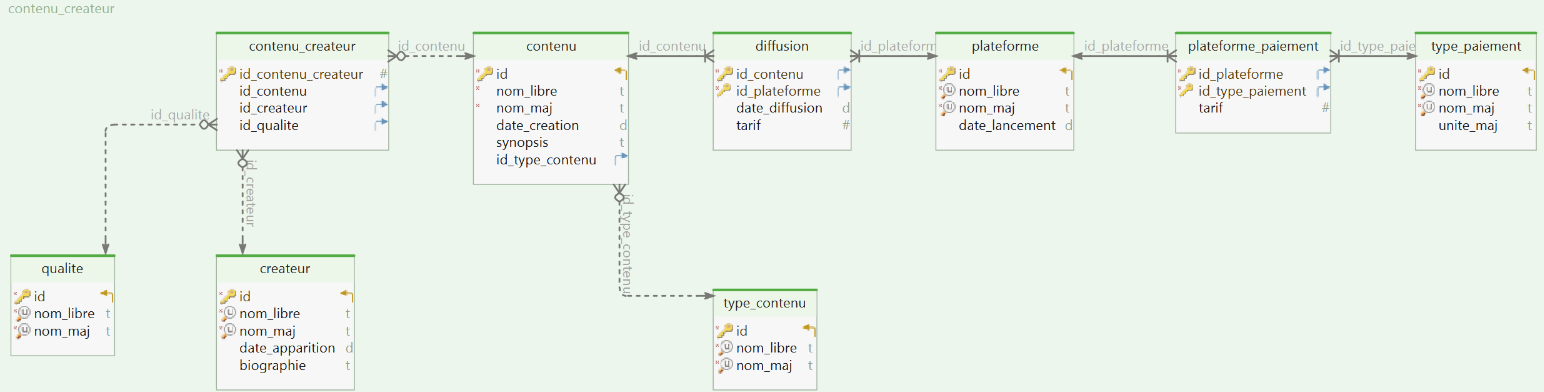
\includegraphics[width=1\linewidth]{image/MR_DUmp.png}
    \caption{MR de la BDD importée}
    \label{fig:enter-label}
\end{figure}

\section{Création de tables}
\subsection{Création}
La commande \texttt{CREATE TABLE} permet de créer une table, exemple :
\begin{lstlisting}[language=SQL]
CREATE TABLE type_plateforme (
    id SERIAL PRIMARY KEY,
    nom_libre TEXT UNIQUE NOT NULL,
    nom_maj TEXT UNIQUE NOT NULL
);
\end{lstlisting}

\subsection{cascade des attributs}
Plusieurs types d'attributs peuvent être utilisés :
\begin{enumerate}
    \item \texttt{TEXT} : Simple texte
    \item \texttt{SERIAL} : Un entier s'incrémentant à chaque nouveau tuple
    \item \texttt{INT} : Un entier
\end{enumerate}

\subsection{Contraintes}
\subsubsection{Contraintes classiques}
\begin{enumerate}
    \item \texttt{PRIMARY KEY} : Contrainte de clé primaire
    \item \texttt{UNIQUE} : Unicité de l'attribut
    \item \texttt{NOT NULL} : Existence de l'attribut
\end{enumerate}

\subsubsection{\texttt{PRIMARY KEY} sur plusieurs attributs}
\begin{lstlisting}[language=SQL]
PRIMARY KEY (<attributPK1>, <attributPK2>)
\end{lstlisting}

\subsubsection{Ajouter \texttt{PRIMARY KEY} après}
\begin{lstlisting}[language=SQL]
ALTER TABLE plateforme
ADD CONSTRAINT plateforme_pkey PRIMARY KEY (id);
\end{lstlisting}

\subsection{Contrainte de clé étrangère}
Pour créer une contrainte de clé étrangère, on commence par créer l'attribut s'il n'existe pas, puis on crée la contrainte et on ajoute également les comportements en cascade :

\begin{lstlisting}[language=SQL]
ALTER TABLE plateforme ADD COLUMN id_type_plateforme INT;

ALTER TABLE plateforme ADD CONSTRAINT

fk_id_type_plateforme FOREIGN KEY(id_type_plateforme)
REFERENCES type_plateforme(id)

ON UPDATE CASCADE
ON DELETE SET NULL;
\end{lstlisting}

\subsubsection{Suppression en cascade}
Doit être utilisé pour les tables tampons
\begin{lstlisting}[language=SQL]
ON DELETE CASCADE
\end{lstlisting}

\subsubsection{Mettre à nul lors de la suppression}
\begin{lstlisting}[language=SQL]
ON DELETE SET NULL
\end{lstlisting}

\subsubsection{Mettre à une valeur par défaut lors de la suppression}
\begin{lstlisting}[language=SQL]
ON DELETE SET DEFAULT
\end{lstlisting}

\subsubsection{Mettre à jour en cascade}
\begin{lstlisting}[language=SQL]
ON UPDATE CASCADE
\end{lstlisting}

\subsubsection{Exemple de création d'une table tampon}
\begin{lstlisting}[language=SQL]
CREATE TABLE contenu_genre(
    id_contenu INT,
    id_genre INT,
    PRIMARY KEY (id_contenu, id_genre)
);

ALTER TABLE contenu_genre ADD CONSTRAINT pk_id_contenu
FOREIGN KEY(id_contenu)
REFERENCES contenu(id)

ON UPDATE CASCADE
ON DELETE CASCADE;

ALTER TABLE contenu_genre ADD CONSTRAINT pk_id_genre
FOREIGN KEY(id_genre)
REFERENCES genre(id)

ON UPDATE CASCADE
ON DELETE CASCADE;
\end{lstlisting}

\section{Insertion et mise à jour des données}
\subsection{Insertion de données}
Exemple d'insertion de plusieurs données :
\begin{lstlisting}[language=SQL]
INSERT INTO type_plateforme (nom_libre)
VALUES ('Streaming Vidéo'), ('Gaming');
\end{lstlisting}

\subsection{Mise à jour des données}
Exemple de mise à jour des données :
\begin{lstlisting}[language=SQL]
UPDATE plateforme SET id_type_plateforme = 1  WHERE nom_maj != 'STEAM';
UPDATE plateforme SET id_type_plateforme = 2 WHERE nom_maj = 'STEAM';
\end{lstlisting}

\subsection{Manipulation date}
Exemple manipulation date : \texttt{'YYYY-MM-DD'}
\begin{lstlisting}[language=SQL]
INSERT INTO diffusion (id_contenu, id_plateforme, date_diffusion, tarif) VALUES (2, 2, '2000-04-05', 25)
\end{lstlisting}

\subsection{Supprimer des données}
\subsubsection{Supprimer toutes les données}
\begin{lstlisting}[language=SQL]
DELETE FROM <nom_table>
\end{lstlisting}

\subsubsection{Supprimer certaines données}
\begin{lstlisting}[language=SQL]
DELETE FROM <nom_table> WHERE <condition>
\end{lstlisting}

\subsection{Insertion depuis fichier \texttt{.csv}}
\textbf{Attention :} Il s'agit de requêtes PSQL et non de requêtes SQL standards.
\begin{lstlisting}[language=SQL]
 \copy nom_table (att1, att2, ...) FROM 'fichier.csv' WITH CSV DELIMITER ';' QUOTE '"'
\end{lstlisting}
\begin{itemize}
    \item \texttt{WITH} introduit les options de l'import
    \item \texttt{CSV} indique qu'il s'agit d'un fichier CSV
    \item \texttt{DELIMITER 'c'} indique que le caractère c est utilisé comme délimiteur de champ (en général ; ou ,)
    \item  \texttt{QUOTE 'c'} indique que le caractère c est utilisé comme délimiteur de chaîne (en général ")
\end{itemize}

\subsubsection{Avec headers}
\begin{lstlisting}[language=SQL]
 \copy nom_table (att1, att2, ...) FROM 'fichier.csv' WITH CSV HEADER DELIMITER ';' QUOTE '"'
\end{lstlisting}

\subsubsection{Exemples}
\begin{lstlisting} [language=SQL]
\copy contenu_genre (id_contenu, id_genre) FROM 'C:/Users/tcade/Downloads/contenu_genre.csv' WITH CSV HEADER DELIMITER ';' QUOTE '"';
\end{lstlisting}

\begin{lstlisting}[language=SQL]
\copy createur (nom_libre, date_apparition, biographie) FROM 'C:/Users/tcade/Downloads/contenu_genre.csv' WITH CSV HEADER DELIMITER ';' QUOTE '"';
\end{lstlisting}

\chapter{Programmation}
\minitoc

\section{Commandes de base}
\subsection{Documentation}
\href{https://docs.postgresql.fr/12/plpgsql.html}{https://docs.postgresql.fr/12/plpgsql.html}

\subsection{Exécuter une fonction}
\begin{lstlisting}[language=SQL]
SELECT fonction()
\end{lstlisting}

\subsection{Supprimer une fonction}
\begin{lstlisting}[language=SQL]
DROP FUNCTION get_max_genre_contenu();
\end{lstlisting}

\subsection{Affectation}
\begin{lstlisting}[language=SQL]
...
DECLARE
var1 INT : 2; --Exemple de déclaration
...

var2 := var3; --Exemple d'affectation
\end{lstlisting}

\subsection{Vider un tableau}
\begin{lstlisting}[language=SQL]
tab_attribut := ARRAY[]::TEXT[];
\end{lstlisting}

\subsection{Spécifier dynamiquement le nom d'une table ou attribut}
Pour spécifier dynamiquement le nom d'une table ou d'une colonne dans la partie FROM ou SELECT de la requête, exemple avec un INTO à la fin de la requête :
\begin{lstlisting}[language=SQL]
EXECUTE format('UPDATE %I SET %I = %L WHERE %I = %L', nom_table, nom_colonne, valeur_colonne, condition_colonne, condition_valeur);
\end{lstlisting}
\begin{itemize}
    \item \texttt{\%I} est utilisé pour les identifiants (comme les noms de tables ou de colonnes) et assure que les noms sont correctement échappés
    \item \texttt{\%L} est utilisé pour les valeurs littérales et s'occupe de les entourer d'apostrophes et d'échapper les apostrophes internes si nécessaire
\end{itemize}

\subsection{Exécuter une requête sans résultat}
Si on ne souhaite pas récupérer le résultat d'une requête SQL, on place le mot-clé \texttt{PERFORM} en amont. Exemple :

\begin{lstlisting}[language=SQL]
PERFOM SELECT * FROM contenu;
\end{lstlisting}

\subsection{Récupérer une ligne de résultat de requête}
On peut placer le retour d'une ligne d'une requête \texttt{SELECT, INSERT, UPDATE, DELETE} dans une variable de type \texttt{RECORD, ROW} ou une liste de variables scalaires. Si la clause "STRICT" est spécifiée, la requête doit renvoyer exactement une ligne. Sinon, la variable "cible" sera configurée avec la première ligne renvoyée par la requête ou à NULL si la requête n'a renvoyé aucune ligne. Toute ligne résultat après la première ligne est annulée. Exemple :
\begin{lstlisting}[language=SQL]
SELECT * INTO monrec FROM emp WHERE nom = mon_nom;

SELECT * INTO STRICT monrec FROM emp WHERE nom = mon_nom;
\end{lstlisting}

\subsection{Récupérer un tableau du résultat d'une requête}
\begin{lstlisting}[language=SQL]
CREATE OR REPLACE FUNCTION liste_genre_contenu (contenu TEXT)
RETURNS TEXT[] AS
$$
DECLARE
    -- Variables
    liste TEXT[];
BEGIN
    -- Requête
    SELECT ARRAY(
        --Votre requete
    ) INTO liste;
    
    -- Retour
    RETURN liste;
END ;
$$
LANGUAGE plpgsql;

\end{lstlisting}

\subsection{Spécifier dynamiquement le nom d'une table ou attribut}
Pour spécifier dynamiquement le nom d'une table ou d'une colonne dans la partie FROM ou SELECT de la requête, exemple avec un INTO à la fin de la requête :
\begin{lstlisting}[language=SQL]
EXECUTE format('SELECT ARRAY(SELECT %I FROM %I)', current_attribut_libre, current_table) INTO tab_text_libre;
\end{lstlisting}

\subsection{\texttt{IF}}
\begin{lstlisting}[language=SQL]
IF nombre = 0 THEN
    resultat := 'zero';
ELSIF nombre > 0 THEN
    resultat := 'positif';
ELSIF nombre < 0 THEN
    resultat := 'negatif';
ELSE
    -- hmm, la seule possibilité est que le nombre soit NULL
    resultat := 'NULL';
END IF;
\end{lstlisting}

\subsection{\texttt{CASE}}
\begin{lstlisting}[language=SQL]
CASE
    WHEN x BETWEEN 0 AND 10 THEN
        msg := 'valeur entre zéro et dix';
    WHEN x BETWEEN 11 AND 20 THEN
        msg := 'valeur entre onze et vingt';
    ELSE
        NULL;
END CASE;
\end{lstlisting}

\subsection{\texttt{WHILE}}
\begin{lstlisting}[language=SQL]
WHILE montant_possede > 0 AND balance_cadeau > 0 LOOP
    -- quelques traitements ici
END LOOP;
\end{lstlisting}

\subsection{Boucler dans une requête}
\begin{lstlisting}[language=SQL]
CREATE FUNCTION rafraichir_vuemat() RETURNS integer AS $$
DECLARE
    vues_mat RECORD;
BEGIN
    RAISE NOTICE 'Rafraichissement de toutes les vues matérialisées...';

    FOR mviews IN
       SELECT n.nspname AS mv_schema,
              c.relname AS mv_name,
              pg_catalog.pg_get_userbyid(c.relowner) AS owner
         FROM pg_catalog.pg_class c
    LEFT JOIN pg_catalog.pg_namespace n ON (n.oid = c.relnamespace)
        WHERE c.relkind = 'm'
     ORDER BY 1
    LOOP

        -- Maintenant "mviews" contient un enregistrement avec les informations sur la vue matérialisée

        RAISE NOTICE 'Rafraichissement de la vue matérialisée %.% (propriétaire : %)...',
                     quote_ident(mviews.mv_schema),
                     quote_ident(mviews.mv_name),
                     quote_ident(mviews.owner);
        EXECUTE format('REFRESH MATERIALIZED VIEW %I.%I', mviews.mv_schema, mviews.mv_name);
    END LOOP;

    RAISE NOTICE 'Fin du rafraichissement des vues matérialisées.';
    RETURN 1;
END;
$$ LANGUAGE plpgsql;
\end{lstlisting}

\subsection{Boucler dans un tableau}
\begin{lstlisting}[language=SQL]
CREATE FUNCTION somme(int[]) RETURNS int8 AS $$
DECLARE
  s int8 := 0;
  x int;
BEGIN
  FOREACH x IN ARRAY $1
  LOOP
    s := s + x;
  END LOOP;
  RETURN s;
END;
$$ LANGUAGE plpgsql;
\end{lstlisting}

\subsection{\texttt{RAISE EXCEPTION}}
Lorsqu'une exception est déclenchée avec RAISE EXCEPTION, PostgreSQL interrompt l'exécution du bloc courant de PL/pgSQL et remonte dans la pile d'appel jusqu'à trouver un bloc englobant équipé d'une gestion d'exception (EXCEPTION). Si aucune gestion d'exception n'est trouvée, la transaction en cours est annulée. Exemple :
\begin{lstlisting}[language=SQL]
DO $$
BEGIN
    -- Tente d'exécuter un code qui pourrait échouer
    RAISE EXCEPTION 'Ceci est un message d''erreur personnalisé.';
EXCEPTION
    WHEN OTHERS THEN
        -- Gestion de l'erreur, peut-être en enregistrant l'erreur ou en effectuant une autre action corrective.
        RAISE NOTICE 'Une erreur a été interceptée et gérée.';
END $$;
\end{lstlisting}

\subsection{\texttt{RAISE NOTICE}}
Une instruction "raise notice" est utilisée pour générer un message au niveau INFO lors de l'exécution d'une fonction ou d'un bloc de code. Elle est principalement utilisée à des fins de débogage et d'information, exemple :
\begin{lstlisting}[language=SQL]
CREATE OR REPLACE FUNCTION example_function() RETURNS VOID AS $$
BEGIN
  -- Faire quelque chose
  RAISE NOTICE 'Ceci est un message de notice'; --Texte
  RAISE NOTICE '%', raise_text; --Avec une variable
  RAISE NOTICE 'message', variables; --Avec message
END;
$$ LANGUAGE plpgsql;
\end{lstlisting}

\subsection{Transformer un tableau en texte}
\begin{lstlisting}[language=SQL]
liste_retour := ARRAY_TO_STRING (liste, ', ');
\end{lstlisting}

\section{Fonction}

\subsection{Canevas}
\begin{lstlisting}[language=SQL]
CREATE OR REPLACE FUNCTION nom_fonction (arg1 IN TYPE)
RETURNS void AS

$$
DECLARE
-- Variables
ma_variable TYPE ;

--Algorithme
BEGIN

END;
$$

LANGUAGE plpgsql;
\end{lstlisting}

\subsection{Exemples}

\subsubsection{Nombre de contenus diffusés par plateforme}
\begin{lstlisting}[language=SQL]
CREATE OR REPLACE FUNCTION nombre_contenus_par_plateforme (id INT)
RETURNS INT AS

$$
DECLARE
-- Variables
NBR INT ;

-- Algorithme
BEGIN
	--Requête
	SELECT
		COUNT (id_contenu) INTO STRICT NBR
	FROM diffusion
	WHERE id_plateforme = id;
	
	--Retour
	RETURN NBR;
END ;
$$

LANGUAGE plpgsql ;
\end{lstlisting}

\subsubsection{Liste des genre d'un contenu}
\begin{lstlisting}[language=SQL]
CREATE OR REPLACE FUNCTION liste_genre_contenu (contenu TEXT)
RETURNS TEXT AS
$$
DECLARE
    -- Variables
    liste TEXT[];
	liste_retour TEXT;
BEGIN
    -- Requête
    SELECT ARRAY(
        SELECT g.nom_libre
        FROM genre AS g
        INNER JOIN contenu_genre AS cg ON cg.id_genre = g.id
        INNER JOIN contenu AS c ON c.id = cg.id_contenu
        WHERE c.nom_libre LIKE contenu
    ) INTO liste;
    
	--Conversion
	liste_retour := ARRAY_TO_STRING (liste, ', ');
	
    -- Retour
    RETURN liste_retour;
END ;
$$
LANGUAGE plpgsql;
\end{lstlisting}

\subsubsection{Lister les genre les plus occurrents}
\begin{lstlisting}[language=SQL]
CREATE OR REPLACE FUNCTION get_max_genre_contenu ()
RETURNS TEXT AS
$$
DECLARE
-- Variables
	liste TEXT[];
	liste_retour TEXT;

-- Algorithme
BEGIN
	SELECT ARRAY(
		SELECT
			genre.nom_libre AS "genre"
			FROM(
				SELECT
					COUNT(id_contenu) AS "nbr_contenu", 
					id_genre
				FROM contenu_genre 
				GROUP BY id_genre
			) AS query_count --Craie une table |id_genre|nbr_apparition|
				INNER JOIN genre ON genre.id = query_count.id_genre --Récupère le nom des genres
			WHERE
				query_count.nbr_contenu = 
					(SELECT 
						MAX(query_max.nbr_contenu) --Récupère le nombre d'appartion du contenu avec le plus d'appration
					FROM(
						SELECT
							COUNT(id_contenu) AS "nbr_contenu", 
							id_genre
						FROM contenu_genre 
						GROUP BY id_genre) AS query_max --Craie une table |id_genre|nbr_apparition|
					)--N'affiche que les genre qui ont un nombre d'apparition égale au nombre d'apparition max
		)INTO liste; --On place dans le tableau les résultats
		
		liste_retour := ARRAY_TO_STRING(liste , ', '); --On place dans texte le tableau
		
		RETURN liste_retour;
END;
$$
LANGUAGE plpgsql ;
\end{lstlisting}

\subsubsection{Afficher un \texttt{RAISE NOTICE}}
\begin{lstlisting}[language=SQL]
CREATE OR REPLACE FUNCTION raise_contenu (id_contenu_to_print INT)
RETURNS void AS
$$
DECLARE
-- Variables
	raise_text TEXT;

-- Algorithme
BEGIN
	SELECT
	CONCAT('Le contenu ', co.nom_libre, ' a été créé le ', co.date_creation, ' par ', STRING_AGG(cr.nom_libre, ', '), '. Voici son synopsis : ', co.synopsis) INTO raise_text
	FROM contenu AS co
		INNER JOIN contenu_createur AS cocr ON co.id = cocr.id_contenu
		INNER JOIN createur AS cr ON cr.id = cocr.id_createur
	WHERE
		co.id = id_contenu_to_print
	GROUP BY
		co.nom_libre,
		co.date_creation,
		co.synopsis;
	
	RAISE NOTICE '%', raise_text;
END;
$$
LANGUAGE plpgsql ;
\end{lstlisting}

\subsubsection{Mise à jour de tous les nom\_libre de la base}
\begin{lstlisting}[language=SQL]
CREATE OR REPLACE FUNCTION set_upper_and_clean_text()
RETURNS VOID AS
$$
DECLARE
    tab_table TEXT[];
    tab_attribut TEXT[];
    current_table TEXT;
    current_attribut TEXT;
    current_attribut_libre TEXT;
    tab_text_libre TEXT[];
	current_text_libre TEXT;
    text_maj TEXT;
BEGIN
    -- Recherche l'ensemble des tables de la BDD
    SELECT ARRAY(
        SELECT table_name
        FROM information_schema.tables
        WHERE table_schema = 'public'
    ) INTO tab_table;
    
    FOREACH current_table IN ARRAY tab_table
    LOOP
        -- Recupère les attributs de la table
        SELECT ARRAY(
            SELECT column_name
            FROM information_schema.columns
            WHERE table_name = current_table
        ) INTO tab_attribut;
		
		--Parcourt les attributs
        FOREACH current_attribut IN ARRAY tab_attribut
        LOOP
            -- Si la table possède un attribut de type "_maj"
            IF current_attribut LIKE '%_maj' THEN
                -- Récupère le nom de l'attribut de type '_libre'
                FOREACH current_attribut_libre IN ARRAY tab_attribut
                LOOP
                    IF current_attribut_libre LIKE '%_libre' THEN
                        -- Recupere les attributs libres
                        EXECUTE format('SELECT ARRAY(SELECT %I FROM %I)', current_attribut_libre, current_table) INTO tab_text_libre;
                        
						FOREACH current_text_libre IN ARRAY tab_text_libre
        				LOOP
							--Applique la fonction pour formater le texte
							text_maj = upper_and_clean_text(current_text_libre, TRUE);
							
							--Update la table
							EXECUTE format('UPDATE %I SET %I = %L WHERE %I = %L', current_table, current_attribut, text_maj, current_attribut_libre, current_text_libre);
						END LOOP;
                    END IF;
                END LOOP;
            END IF;
        END LOOP;
    END LOOP;
END;
$$
LANGUAGE plpgsql;
\end{lstlisting}

\section{Trigger}\label{trigger}
Un trigger, également appelé déclencheur, permet d’exécuter un ensemble d’instructions SQL juste après un événement, telles que des requêtes \texttt{INSERT} ou \texttt{UPDATE}. Cela permet de faciliter et d’automatiser des actions au sein d’un Système de Gestion de Base de Données (SGBD).

\subsection{Canevas}
\begin{lstlisting}[language=SQL]
CREATE OR REPLACE FUNCTION trigger_before_update_insert_nomfonction ()

RETURNS TRIGGER AS
$nomfonction$

DECLARE
--Variables
var TYPE ;

--Alrgorithme
BEGIN
	--Instructions

	-- Retour du tuple NEW (type RECORD) qui doit etre insere ou mis a jour
	RETURN NEW;
END;

$nomfonction$

LANGUAGE plpgsql;

--Creation du trigger
CREATE TRIGGER trig_nomfonction AFTER INSERT OR UPDATE ON une_table
FOR EACH ROW EXECUTE PROCEDURE trigger_before_update_insert_nomfonction ();
\end{lstlisting}

\subsection{Supprimer un trigger}
\begin{lstlisting}[language=SQL]
DROP TRIGGER IF EXISTS trig_check_date_diffusion ON diffusion; --Pour supprimer le trigger sur une table
DROP FUNCTION IF EXISTS trigger_check_date_diffusion; --Pour supprimer la fonction/procédure
\end{lstlisting}
\textbf{Attention :} Il faut différencier le trigger de la fonction

\subsection{Manipuler les attributs}
Les attributs du tuple à créer sont passés au trigger par l'élément \texttt{NEW}. Exemple :
\begin{lstlisting}[language=SQL]
IF NEW.nom_libre IS NOT NULL THEN
	NEW.nom_maj = upper_and_clean_text (NEW.nom_libre, TRUE) ;
END IF;
\end{lstlisting}

\subsection{Exemples : Vérification cohérence de dates}
\begin{lstlisting}[language=SQL]
CREATE OR REPLACE FUNCTION trigger_check_date_diffusion ()

RETURNS TRIGGER AS
$check_date_diffusion$

DECLARE
--Variables
date_creation_contenu DATE;

--Alrgorithme
BEGIN
	--Recupere la date de creation du contenu
	SELECT date_creation INTO date_creation_contenu FROM contenu WHERE id = NEW.id_contenu;
	
	--Si la date de diffusion est sup à la date de création on annule la transaction
	IF NEW.date_diffusion > date_creation_contenu THEN
		RAISE EXCEPTION 'Erreur : la date de diffusion ne peut pas être supérieure à la date de creation du contenu';
	END IF;
	
	--Si non on continue la transaction
	RETURN NEW;
END;

$check_date_diffusion$

LANGUAGE plpgsql;

CREATE TRIGGER trig_check_date_diffusion AFTER INSERT OR UPDATE ON diffusion

FOR EACH ROW EXECUTE PROCEDURE trigger_check_date_diffusion ();
\end{lstlisting}

\subsection{Trigger sur une vue}
\begin{lstlisting}[language=SQL]
CREATE OR REPLACE FUNCTION trigger_before_insert_view_plateforme_type ()

RETURNS TRIGGER AS
$trig_view_plateforme_type$

DECLARE
--Variables
id_type_plateforme_get INT;

--Alrgorithme
BEGIN
	--Verifie qu'aucun attribut est nul
	IF NEW.plateforme IS NULL OR NEW.type_plateforme IS NULL THEN
		RAISE EXCEPTION 'Error : Les attributs sont non nuls';
	END IF;
	
	--Verifie si le type de plateforme existe si non le crée
	IF NOT EXISTS (SELECT * FROM type_plateforme WHERE nom_maj LIKE upper_and_clean_text(NEW.type_plateforme, TRUE)) THEN
		INSERT INTO type_plateforme (nom_libre) VALUES (NEW.type_plateforme);
	END IF;
	
	--Recupere l'id du type de la plateforme
	SELECT id INTO id_type_plateforme_get FROM type_plateforme WHERE nom_maj LIKE upper_and_clean_text(NEW.type_plateforme, TRUE);
	
	--Verifie si la plateforme existe
	IF NOT EXISTS (SELECT * FROM plateforme WHERE nom_maj LIKE upper_and_clean_text(NEW.plateforme, TRUE)) THEN
		--N'existe pas : On insert dans la table une nouvelle plateforme
		INSERT INTO plateforme(nom_libre, date_lancement, id_type_plateforme) VALUES(NEW.plateforme, NEW.date_lancement, id_type_plateforme_get);
	ELSE
		--Existe : On met à jour son type_plateforme
		UPDATE plateforme SET id_type_plateforme = id_type_plateforme_get WHERE nom_maj LIKE upper_and_clean_text(NEW.plateforme, TRUE);
		
		--On verifie que sa date de lancement concorde si elle n'est pas nulle
		IF NEW.date_lancement IS NOT NULL THEN
			IF ((SELECT date_lancement FROM plateforme WHERE nom_maj LIKE upper_and_clean_text(NEW.plateforme, TRUE)) != NEW.date_lancement) OR ((SELECT date_lancement FROM plateforme WHERE nom_maj LIKE upper_and_clean_text(NEW.plateforme, TRUE)) IS NULL) THEN
				--La date ne concorde pas : On met à jour
				UPDATE plateforme SET date_lancement = NEW.date_lancement WHERE nom_libre LIKE NEW.plateforme;
			END IF;
		END IF;
	END IF;
		
	--Trigger sur vue => Retourne NULL
	RETURN NULL;
END;

$trig_view_plateforme_type$
LANGUAGE plpgsql;

--Creation du trigger
CREATE TRIGGER trig_view_plateforme_type INSTEAD OF INSERT OR UPDATE ON vue_plateforme_type
FOR EACH ROW EXECUTE PROCEDURE trigger_before_insert_view_plateforme_type ();
\end{lstlisting}
\textbf{Attention :} Un trigger sur une vue retourne \texttt{NULL}\\
\textbf{Attention :} La création du trigger est spécifique à une vue\\

\subsection{Remplir des tables avec une vue et un trigger}

En fonction des règles définies par un trigger, il est possible de mettre à jour ou de compléter une vue afin d'actualiser ou de compléter d'autres tables. Exemple :
\begin{lstlisting}[language=SQL]
INSERT INTO vue_contenu_genre_type(contenu, date_creation, synopsis, type_contenu, genre)
VALUES('Taxi4', '2007-01-01', 'Suite de Taxi3', 'film', 'action')
\end{lstlisting}

Cette requête crée dans la table \textit{contenu} \textit{Taxi4}, dans la table \textit{genre} \textit{action} et recherche \textit{film} qui existe déja dans la table \textit{type\_contenu} \textit{'film'}. Ils les associent dans les tables \textit{genre\_contenu} et \textit{contenu}.
\begin{lstlisting}[language=SQL]
UPDATE vue_contenu_genre_type 
SET genre = 'comédie' 
WHERE contenu = 'Taxi4'
\end{lstlisting}

Cette requête modifie le genre en \textit{comédie} tout en créant le genre \textit{comédie} dans la table \textit{genre}. Pour rajouter un genre il faut créer un nouveau tuple. \textbf{Attention :} On utilise l'id conformément à la documentation du trigger : 
\begin{lstlisting}[language=SQL]
INSERT INTO vue_contenu_genre_type(id, date_creation, synopsis, type_contenu, genre)
VALUES(9, '2007-01-01', 'Suite de Taxi3', 'film', 'action')
\end{lstlisting}